\documentclass[a4paper, 12pt, twocolumn, twoside]{report} 

%%%%%%%%%%%%%%%%%%%%%%%%%%%%%%%%%
% PACKAGE IMPORTS
%%%%%%%%%%%%%%%%%%%%%%%%%%%%%%%%%


\usepackage[tmargin=2cm,rmargin=1in,lmargin=1in,margin=0.85in,bmargin=2cm,footskip=.2in]{geometry}
\usepackage{amsmath,amsfonts,amsthm,amssymb,mathtools}
\usepackage[varbb]{newpxmath}
\usepackage{xfrac}
\usepackage[makeroom]{cancel}
\usepackage{mathtools}
\usepackage{bookmark}
\usepackage{enumitem}
\usepackage{hyperref,theoremref}
\hypersetup{
	pdftitle={Assignment},
	colorlinks=true, linkcolor=doc!90,
	bookmarksnumbered=true,
	bookmarksopen=true
}
\usepackage[most,many,breakable]{tcolorbox}
\usepackage{xcolor}
\usepackage{varwidth}
\usepackage{varwidth}
\usepackage{etoolbox}
%\usepackage{authblk}
\usepackage{nameref}
\usepackage{multicol,array}
\usepackage{tikz-cd}
\usepackage[ruled,vlined,linesnumbered]{algorithm2e}
\usepackage{comment} % enables the use of multi-line comments (\ifx \fi) 
\usepackage{import}
\usepackage{xifthen}
\usepackage{pdfpages}
\usepackage{transparent}

\newcommand\mycommfont[1]{\footnotesize\ttfamily\textcolor{blue}{#1}}
\SetCommentSty{mycommfont}
\newcommand{\incfig}[1]{%
    \def\svgwidth{\columnwidth}
    \import{./figures/}{#1.pdf_tex}
}

\usepackage{tikzsymbols}
\renewcommand\qedsymbol{$\Laughey$}


%\usepackage{import}
%\usepackage{xifthen}
%\usepackage{pdfpages}
%\usepackage{transparent}


%%%%%%%%%%%%%%%%%%%%%%%%%%%%%%
% SELF MADE COLORS
%%%%%%%%%%%%%%%%%%%%%%%%%%%%%%



\definecolor{myg}{RGB}{56, 140, 70}
\definecolor{myb}{RGB}{45, 111, 177}
\definecolor{myr}{RGB}{199, 68, 64}
\definecolor{mytheorembg}{HTML}{F2F2F9}
\definecolor{mytheoremfr}{HTML}{00007B}
\definecolor{mylenmabg}{HTML}{FFFAF8}
\definecolor{mylenmafr}{HTML}{983b0f}
\definecolor{mypropbg}{HTML}{f2fbfc}
\definecolor{mypropfr}{HTML}{191971}
\definecolor{myexamplebg}{HTML}{F2FBF8}
\definecolor{myexamplefr}{HTML}{88D6D1}
\definecolor{myexampleti}{HTML}{2A7F7F}
\definecolor{mydefinitbg}{HTML}{E5E5FF}
\definecolor{mydefinitfr}{HTML}{3F3FA3}
\definecolor{notesgreen}{RGB}{0,162,0}
\definecolor{myp}{RGB}{197, 92, 212}
\definecolor{mygr}{HTML}{2C3338}
\definecolor{myred}{RGB}{127,0,0}
\definecolor{myyellow}{RGB}{169,121,69}
\definecolor{myexercisebg}{HTML}{F2FBF8}
\definecolor{myexercisefg}{HTML}{88D6D1}


%%%%%%%%%%%%%%%%%%%%%%%%%%%%
% TCOLORBOX SETUPS
%%%%%%%%%%%%%%%%%%%%%%%%%%%%

\setlength{\parindent}{1cm}
%================================
% THEOREM BOX
%================================

\tcbuselibrary{theorems,skins,hooks}
\newtcbtheorem[number within=section]{Theorem}{Theorem}
{%
	enhanced,
	breakable,
	colback = mytheorembg,
	frame hidden,
	boxrule = 0sp,
	borderline west = {2pt}{0pt}{mytheoremfr},
	sharp corners,
	detach title,
	before upper = \tcbtitle\par\smallskip,
	coltitle = mytheoremfr,
	fonttitle = \bfseries\sffamily,
	description font = \mdseries,
	separator sign none,
	segmentation style={solid, mytheoremfr},
}
{th}

\tcbuselibrary{theorems,skins,hooks}
\newtcbtheorem[number within=chapter]{theorem}{Theorem}
{%
	enhanced,
	breakable,
	colback = mytheorembg,
	frame hidden,
	boxrule = 0sp,
	borderline west = {2pt}{0pt}{mytheoremfr},
	sharp corners,
	detach title,
	before upper = \tcbtitle\par\smallskip,
	coltitle = mytheoremfr,
	fonttitle = \bfseries\sffamily,
	description font = \mdseries,
	separator sign none,
	segmentation style={solid, mytheoremfr},
}
{th}


\tcbuselibrary{theorems,skins,hooks}
\newtcolorbox{Theoremcon}
{%
	enhanced
	,breakable
	,colback = mytheorembg
	,frame hidden
	,boxrule = 0sp
	,borderline west = {2pt}{0pt}{mytheoremfr}
	,sharp corners
	,description font = \mdseries
	,separator sign none
}

%================================
% Corollery
%================================
\tcbuselibrary{theorems,skins,hooks}
\newtcbtheorem[number within=section]{Corollary}{Corollary}
{%
	enhanced
	,breakable
	,colback = myp!10
	,frame hidden
	,boxrule = 0sp
	,borderline west = {2pt}{0pt}{myp!85!black}
	,sharp corners
	,detach title
	,before upper = \tcbtitle\par\smallskip
	,coltitle = myp!85!black
	,fonttitle = \bfseries\sffamily
	,description font = \mdseries
	,separator sign none
	,segmentation style={solid, myp!85!black}
}
{th}
\tcbuselibrary{theorems,skins,hooks}
\newtcbtheorem[number within=chapter]{corollary}{Corollary}
{%
	enhanced
	,breakable
	,colback = myp!10
	,frame hidden
	,boxrule = 0sp
	,borderline west = {2pt}{0pt}{myp!85!black}
	,sharp corners
	,detach title
	,before upper = \tcbtitle\par\smallskip
	,coltitle = myp!85!black
	,fonttitle = \bfseries\sffamily
	,description font = \mdseries
	,separator sign none
	,segmentation style={solid, myp!85!black}
}
{th}


%================================
% LENMA
%================================

\tcbuselibrary{theorems,skins,hooks}
\newtcbtheorem[number within=section]{Lenma}{Lenma}
{%
	enhanced,
	breakable,
	colback = mylenmabg,
	frame hidden,
	boxrule = 0sp,
	borderline west = {2pt}{0pt}{mylenmafr},
	sharp corners,
	detach title,
	before upper = \tcbtitle\par\smallskip,
	coltitle = mylenmafr,
	fonttitle = \bfseries\sffamily,
	description font = \mdseries,
	separator sign none,
	segmentation style={solid, mylenmafr},
}
{th}

\tcbuselibrary{theorems,skins,hooks}
\newtcbtheorem[number within=chapter]{lenma}{Lenma}
{%
	enhanced,
	breakable,
	colback = mylenmabg,
	frame hidden,
	boxrule = 0sp,
	borderline west = {2pt}{0pt}{mylenmafr},
	sharp corners,
	detach title,
	before upper = \tcbtitle\par\smallskip,
	coltitle = mylenmafr,
	fonttitle = \bfseries\sffamily,
	description font = \mdseries,
	separator sign none,
	segmentation style={solid, mylenmafr},
}
{th}


%================================
% PROPOSITION
%================================

\tcbuselibrary{theorems,skins,hooks}
\newtcbtheorem[number within=section]{Prop}{Proposition}
{%
	enhanced,
	breakable,
	colback = mypropbg,
	frame hidden,
	boxrule = 0sp,
	borderline west = {2pt}{0pt}{mypropfr},
	sharp corners,
	detach title,
	before upper = \tcbtitle\par\smallskip,
	coltitle = mypropfr,
	fonttitle = \bfseries\sffamily,
	description font = \mdseries,
	separator sign none,
	segmentation style={solid, mypropfr},
}
{th}

\tcbuselibrary{theorems,skins,hooks}
\newtcbtheorem[number within=chapter]{prop}{Proposition}
{%
	enhanced,
	breakable,
	colback = mypropbg,
	frame hidden,
	boxrule = 0sp,
	borderline west = {2pt}{0pt}{mypropfr},
	sharp corners,
	detach title,
	before upper = \tcbtitle\par\smallskip,
	coltitle = mypropfr,
	fonttitle = \bfseries\sffamily,
	description font = \mdseries,
	separator sign none,
	segmentation style={solid, mypropfr},
}
{th}


%================================
% CLAIM
%================================

\tcbuselibrary{theorems,skins,hooks}
\newtcbtheorem[number within=section]{claim}{Claim}
{%
	enhanced
	,breakable
	,colback = myg!10
	,frame hidden
	,boxrule = 0sp
	,borderline west = {2pt}{0pt}{myg}
	,sharp corners
	,detach title
	,before upper = \tcbtitle\par\smallskip
	,coltitle = myg!85!black
	,fonttitle = \bfseries\sffamily
	,description font = \mdseries
	,separator sign none
	,segmentation style={solid, myg!85!black}
}
{th}



%================================
% Exercise
%================================

\tcbuselibrary{theorems,skins,hooks}
\newtcbtheorem[number within=section]{Exercise}{Exercise}
{%
	enhanced,
	breakable,
	colback = myexercisebg,
	frame hidden,
	boxrule = 0sp,
	borderline west = {2pt}{0pt}{myexercisefg},
	sharp corners,
	detach title,
	before upper = \tcbtitle\par\smallskip,
	coltitle = myexercisefg,
	fonttitle = \bfseries\sffamily,
	description font = \mdseries,
	separator sign none,
	segmentation style={solid, myexercisefg},
}
{th}

\tcbuselibrary{theorems,skins,hooks}
\newtcbtheorem[number within=chapter]{exercise}{Exercise}
{%
	enhanced,
	breakable,
	colback = myexercisebg,
	frame hidden,
	boxrule = 0sp,
	borderline west = {2pt}{0pt}{myexercisefg},
	sharp corners,
	detach title,
	before upper = \tcbtitle\par\smallskip,
	coltitle = myexercisefg,
	fonttitle = \bfseries\sffamily,
	description font = \mdseries,
	separator sign none,
	segmentation style={solid, myexercisefg},
}
{th}

%================================
% EXAMPLE BOX
%================================

\newtcbtheorem[number within=section]{Example}{Example}
{%
	colback = myexamplebg
	,breakable
	,colframe = myexamplefr
	,coltitle = myexampleti
	,boxrule = 1pt
	,sharp corners
	,detach title
	,before upper=\tcbtitle\par\smallskip
	,fonttitle = \bfseries
	,description font = \mdseries
	,separator sign none
	,description delimiters parenthesis
}
{ex}

\newtcbtheorem[number within=chapter]{example}{Example}
{%
	colback = myexamplebg
	,breakable
	,colframe = myexamplefr
	,coltitle = myexampleti
	,boxrule = 1pt
	,sharp corners
	,detach title
	,before upper=\tcbtitle\par\smallskip
	,fonttitle = \bfseries
	,description font = \mdseries
	,separator sign none
	,description delimiters parenthesis
}
{ex}

%================================
% DEFINITION BOX
%================================

\newtcbtheorem[number within=section]{Definition}{Definition}{enhanced,
	before skip=2mm,after skip=2mm, colback=red!5,colframe=red!80!black,boxrule=0.5mm,
	attach boxed title to top left={xshift=1cm,yshift*=1mm-\tcboxedtitleheight}, varwidth boxed title*=-3cm,
	boxed title style={frame code={
					\path[fill=tcbcolback]
					([yshift=-1mm,xshift=-1mm]frame.north west)
					arc[start angle=0,end angle=180,radius=1mm]
					([yshift=-1mm,xshift=1mm]frame.north east)
					arc[start angle=180,end angle=0,radius=1mm];
					\path[left color=tcbcolback!60!black,right color=tcbcolback!60!black,
						middle color=tcbcolback!80!black]
					([xshift=-2mm]frame.north west) -- ([xshift=2mm]frame.north east)
					[rounded corners=1mm]-- ([xshift=1mm,yshift=-1mm]frame.north east)
					-- (frame.south east) -- (frame.south west)
					-- ([xshift=-1mm,yshift=-1mm]frame.north west)
					[sharp corners]-- cycle;
				},interior engine=empty,
		},
	fonttitle=\bfseries,
	title={#2},#1}{def}
\newtcbtheorem[number within=chapter]{definition}{Definition}{enhanced,
	before skip=2mm,after skip=2mm, colback=red!5,colframe=red!80!black,boxrule=0.5mm,
	attach boxed title to top left={xshift=1cm,yshift*=1mm-\tcboxedtitleheight}, varwidth boxed title*=-3cm,
	boxed title style={frame code={
					\path[fill=tcbcolback]
					([yshift=-1mm,xshift=-1mm]frame.north west)
					arc[start angle=0,end angle=180,radius=1mm]
					([yshift=-1mm,xshift=1mm]frame.north east)
					arc[start angle=180,end angle=0,radius=1mm];
					\path[left color=tcbcolback!60!black,right color=tcbcolback!60!black,
						middle color=tcbcolback!80!black]
					([xshift=-2mm]frame.north west) -- ([xshift=2mm]frame.north east)
					[rounded corners=1mm]-- ([xshift=1mm,yshift=-1mm]frame.north east)
					-- (frame.south east) -- (frame.south west)
					-- ([xshift=-1mm,yshift=-1mm]frame.north west)
					[sharp corners]-- cycle;
				},interior engine=empty,
		},
	fonttitle=\bfseries,
	title={#2},#1}{def}



%================================
% Solution BOX
%================================

\makeatletter
\newtcbtheorem{question}{Question}{enhanced,
	breakable,
	colback=white,
	colframe=myb!80!black,
	attach boxed title to top left={yshift*=-\tcboxedtitleheight},
	fonttitle=\bfseries,
	title={#2},
	boxed title size=title,
	boxed title style={%
			sharp corners,
			rounded corners=northwest,
			colback=tcbcolframe,
			boxrule=0pt,
		},
	underlay boxed title={%
			\path[fill=tcbcolframe] (title.south west)--(title.south east)
			to[out=0, in=180] ([xshift=5mm]title.east)--
			(title.center-|frame.east)
			[rounded corners=\kvtcb@arc] |-
			(frame.north) -| cycle;
		},
	#1
}{def}
\makeatother

%================================
% SOLUTION BOX
%================================

\makeatletter
\newtcolorbox{solution}{enhanced,
	breakable,
	colback=white,
	colframe=myg!80!black,
	attach boxed title to top left={yshift*=-\tcboxedtitleheight},
	title=Solution,
	boxed title size=title,
	boxed title style={%
			sharp corners,
			rounded corners=northwest,
			colback=tcbcolframe,
			boxrule=0pt,
		},
	underlay boxed title={%
			\path[fill=tcbcolframe] (title.south west)--(title.south east)
			to[out=0, in=180] ([xshift=5mm]title.east)--
			(title.center-|frame.east)
			[rounded corners=\kvtcb@arc] |-
			(frame.north) -| cycle;
		},
}
\makeatother

%================================
% Question BOX
%================================

\makeatletter
\newtcbtheorem{qstion}{Question}{enhanced,
	breakable,
	colback=white,
	colframe=mygr,
	attach boxed title to top left={yshift*=-\tcboxedtitleheight},
	fonttitle=\bfseries,
	title={#2},
	boxed title size=title,
	boxed title style={%
			sharp corners,
			rounded corners=northwest,
			colback=tcbcolframe,
			boxrule=0pt,
		},
	underlay boxed title={%
			\path[fill=tcbcolframe] (title.south west)--(title.south east)
			to[out=0, in=180] ([xshift=5mm]title.east)--
			(title.center-|frame.east)
			[rounded corners=\kvtcb@arc] |-
			(frame.north) -| cycle;
		},
	#1
}{def}
\makeatother

\newtcbtheorem[number within=chapter]{wconc}{Wrong Concept}{
	breakable,
	enhanced,
	colback=white,
	colframe=myr,
	arc=0pt,
	outer arc=0pt,
	fonttitle=\bfseries\sffamily\large,
	colbacktitle=myr,
	attach boxed title to top left={},
	boxed title style={
			enhanced,
			skin=enhancedfirst jigsaw,
			arc=3pt,
			bottom=0pt,
			interior style={fill=myr}
		},
	#1
}{def}



%================================
% NOTE BOX
%================================

\usetikzlibrary{arrows,calc,shadows.blur}
\tcbuselibrary{skins}
\newtcolorbox{note}[1][]{%
	enhanced jigsaw,
	colback=gray!20!white,%
	colframe=gray!80!black,
	size=small,
	boxrule=1pt,
	title=\textbf{Note:-},
	halign title=flush center,
	coltitle=black,
	breakable,
	drop shadow=black!50!white,
	attach boxed title to top left={xshift=1cm,yshift=-\tcboxedtitleheight/2,yshifttext=-\tcboxedtitleheight/2},
	minipage boxed title=1.5cm,
	boxed title style={%
			colback=white,
			size=fbox,
			boxrule=1pt,
			boxsep=2pt,
			underlay={%
					\coordinate (dotA) at ($(interior.west) + (-0.5pt,0)$);
					\coordinate (dotB) at ($(interior.east) + (0.5pt,0)$);
					\begin{scope}
						\clip (interior.north west) rectangle ([xshift=3ex]interior.east);
						\filldraw [white, blur shadow={shadow opacity=60, shadow yshift=-.75ex}, rounded corners=2pt] (interior.north west) rectangle (interior.south east);
					\end{scope}
					\begin{scope}[gray!80!black]
						\fill (dotA) circle (2pt);
						\fill (dotB) circle (2pt);
					\end{scope}
				},
		},
	#1,
}

%%%%%%%%%%%%%%%%%%%%%%%%%%%%%%
% SELF MADE COMMANDS
%%%%%%%%%%%%%%%%%%%%%%%%%%%%%%


\newcommand{\thm}[2]{\begin{Theorem}{#1}{}#2\end{Theorem}}
\newcommand{\cor}[2]{\begin{Corollary}{#1}{}#2\end{Corollary}}
\newcommand{\mlenma}[2]{\begin{Lenma}{#1}{}#2\end{Lenma}}
\newcommand{\mprop}[2]{\begin{Prop}{#1}{}#2\end{Prop}}
\newcommand{\clm}[3]{\begin{claim}{#1}{#2}#3\end{claim}}
\newcommand{\wc}[2]{\begin{wconc}{#1}{}\setlength{\parindent}{1cm}#2\end{wconc}}
\newcommand{\thmcon}[1]{\begin{Theoremcon}{#1}\end{Theoremcon}}
\newcommand{\ex}[2]{\begin{Example}{#1}{}#2\end{Example}}
\newcommand{\dfn}[2]{\begin{Definition}[colbacktitle=red!75!black]{#1}{}#2\end{Definition}}
\newcommand{\dfnc}[2]{\begin{definition}[colbacktitle=red!75!black]{#1}{}#2\end{definition}}
\newcommand{\qs}[2]{\begin{question}{#1}{}#2\end{question}}
\newcommand{\pf}[2]{\begin{myproof}[#1]#2\end{myproof}}
\newcommand{\nt}[1]{\begin{note}#1\end{note}}

\newcommand*\circled[1]{\tikz[baseline=(char.base)]{
		\node[shape=circle,draw,inner sep=1pt] (char) {#1};}}
\newcommand\getcurrentref[1]{%
	\ifnumequal{\value{#1}}{0}
	{??}
	{\the\value{#1}}%
}
\newcommand{\getCurrentSectionNumber}{\getcurrentref{section}}
\newenvironment{myproof}[1][\proofname]{%
	\proof[\bfseries #1: ]%
}{\endproof}

\newcommand{\mclm}[2]{\begin{myclaim}[#1]#2\end{myclaim}}
\newenvironment{myclaim}[1][\claimname]{\proof[\bfseries #1: ]}{}

\newcounter{mylabelcounter}

\makeatletter
\newcommand{\setword}[2]{%
	\phantomsection
	#1\def\@currentlabel{\unexpanded{#1}}\label{#2}%
}
\makeatother




\tikzset{
	symbol/.style={
			draw=none,
			every to/.append style={
					edge node={node [sloped, allow upside down, auto=false]{$#1$}}}
		}
}


% deliminators
\DeclarePairedDelimiter{\abs}{\lvert}{\rvert}
\DeclarePairedDelimiter{\norm}{\lVert}{\rVert}

\DeclarePairedDelimiter{\ceil}{\lceil}{\rceil}
\DeclarePairedDelimiter{\floor}{\lfloor}{\rfloor}
\DeclarePairedDelimiter{\round}{\lfloor}{\rceil}

\newsavebox\diffdbox
\newcommand{\slantedromand}{{\mathpalette\makesl{d}}}
\newcommand{\makesl}[2]{%
\begingroup
\sbox{\diffdbox}{$\mathsurround=0pt#1\mathrm{#2}$}%
\pdfsave
\pdfsetmatrix{1 0 0.2 1}%
\rlap{\usebox{\diffdbox}}%
\pdfrestore
\hskip\wd\diffdbox
\endgroup
}
\newcommand{\dd}[1][]{\ensuremath{\mathop{}\!\ifstrempty{#1}{%
\slantedromand\@ifnextchar^{\hspace{0.2ex}}{\hspace{0.1ex}}}%
{\slantedromand\hspace{0.2ex}^{#1}}}}
\ProvideDocumentCommand\dv{o m g}{%
  \ensuremath{%
    \IfValueTF{#3}{%
      \IfNoValueTF{#1}{%
        \frac{\dd #2}{\dd #3}%
      }{%
        \frac{\dd^{#1} #2}{\dd #3^{#1}}%
      }%
    }{%
      \IfNoValueTF{#1}{%
        \frac{\dd}{\dd #2}%
      }{%
        \frac{\dd^{#1}}{\dd #2^{#1}}%
      }%
    }%
  }%
}
\providecommand*{\pdv}[3][]{\frac{\partial^{#1}#2}{\partial#3^{#1}}}
%  - others
\DeclareMathOperator{\Lap}{\mathcal{L}}
\DeclareMathOperator{\Var}{Var} % varience
\DeclareMathOperator{\Cov}{Cov} % covarience
\DeclareMathOperator{\E}{E} % expected

% Since the amsthm package isn't loaded

% I prefer the slanted \leq
\let\oldleq\leq % save them in case they're every wanted
\let\oldgeq\geq
\renewcommand{\leq}{\leqslant}
\renewcommand{\geq}{\geqslant}

% % redefine matrix env to allow for alignment, use r as default
% \renewcommand*\env@matrix[1][r]{\hskip -\arraycolsep
%     \let\@ifnextchar\new@ifnextchar
%     \array{*\c@MaxMatrixCols #1}}


%\usepackage{framed}
%\usepackage{titletoc}
%\usepackage{etoolbox}
%\usepackage{lmodern}


%\patchcmd{\tableofcontents}{\contentsname}{\sffamily\contentsname}{}{}

%\renewenvironment{leftbar}
%{\def\FrameCommand{\hspace{6em}%
%		{\color{myyellow}\vrule width 2pt depth 6pt}\hspace{1em}}%
%	\MakeFramed{\parshape 1 0cm \dimexpr\textwidth-6em\relax\FrameRestore}\vskip2pt%
%}
%{\endMakeFramed}

%\titlecontents{chapter}
%[0em]{\vspace*{2\baselineskip}}
%{\parbox{4.5em}{%
%		\hfill\Huge\sffamily\bfseries\color{myred}\thecontentspage}%
%	\vspace*{-2.3\baselineskip}\leftbar\textsc{\small\chaptername~\thecontentslabel}\\\sffamily}
%{}{\endleftbar}
%\titlecontents{section}
%[8.4em]
%{\sffamily\contentslabel{3em}}{}{}
%{\hspace{0.5em}\nobreak\itshape\color{myred}\contentspage}
%\titlecontents{subsection}
%[8.4em]
%{\sffamily\contentslabel{3em}}{}{}  
%{\hspace{0.5em}\nobreak\itshape\color{myred}\contentspage}



%%%%%%%%%%%%%%%%%%%%%%%%%%%%%%%%%%%%%%%%%%%
% TABLE OF CONTENTS
%%%%%%%%%%%%%%%%%%%%%%%%%%%%%%%%%%%%%%%%%%%

\usepackage{tikz}
\definecolor{doc}{RGB}{0,60,110}
\usepackage{titletoc}
\contentsmargin{0cm}
\titlecontents{chapter}[3.7pc]
{\addvspace{30pt}%
	\begin{tikzpicture}[remember picture, overlay]%
		\draw[fill=doc!60,draw=doc!60] (-7,-.1) rectangle (-0.9,.5);%
		\pgftext[left,x=-3.5cm,y=0.2cm]{\color{white}\Large\sc\bfseries Chapter\ \thecontentslabel};%
	\end{tikzpicture}\color{doc!60}\large\sc\bfseries}%
{}
{}
{\;\titlerule\;\large\sc\bfseries Page \thecontentspage
	\begin{tikzpicture}[remember picture, overlay]
		\draw[fill=doc!60,draw=doc!60] (2pt,0) rectangle (4,0.1pt);
	\end{tikzpicture}}%
\titlecontents{section}[3.7pc]
{\addvspace{2pt}}
{\contentslabel[\thecontentslabel]{2pc}}
{}
{\hfill\small \thecontentspage}
[]
\titlecontents*{subsection}[3.7pc]
{\addvspace{-1pt}\small}
{}
{}
{\ --- \small\thecontentspage}
[ \textbullet\ ][]

\makeatletter
\renewcommand{\tableofcontents}{%
	\chapter*{%
	  \vspace*{-20\p@}%
	  \begin{tikzpicture}[remember picture, overlay]%
		  \pgftext[right,x=15cm,y=0.2cm]{\color{doc!60}\Huge\sc\bfseries \contentsname};%
		  \draw[fill=doc!60,draw=doc!60] (13,-.75) rectangle (20,1);%
		  \clip (13,-.75) rectangle (20,1);
		  \pgftext[right,x=15cm,y=0.2cm]{\color{white}\Huge\sc\bfseries \contentsname};%
	  \end{tikzpicture}}%
	\@starttoc{toc}}
\makeatother

%From M275 "Topology" at SJSU
\newcommand{\id}{\mathrm{id}}
\newcommand{\taking}[1]{\xrightarrow{#1}}
\newcommand{\inv}{^{-1}}

%From M170 "Introduction to Graph Theory" at SJSU
\DeclareMathOperator{\diam}{diam}
\DeclareMathOperator{\ord}{ord}
\newcommand{\defeq}{\overset{\mathrm{def}}{=}}

%From the USAMO .tex files
\newcommand{\ts}{\textsuperscript}
\newcommand{\dg}{^\circ}
\newcommand{\ii}{\item}

% % From Math 55 and Math 145 at Harvard
% \newenvironment{subproof}[1][Proof]{%
% \begin{proof}[#1] \renewcommand{\qedsymbol}{$\blacksquare$}}%
% {\end{proof}}

\newcommand{\liff}{\leftrightarrow}
\newcommand{\lthen}{\rightarrow}
\newcommand{\opname}{\operatorname}
\newcommand{\surjto}{\twoheadrightarrow}
\newcommand{\injto}{\hookrightarrow}
\newcommand{\On}{\mathrm{On}} % ordinals
\DeclareMathOperator{\img}{im} % Image
\DeclareMathOperator{\Img}{Im} % Image
\DeclareMathOperator{\coker}{coker} % Cokernel
\DeclareMathOperator{\Coker}{Coker} % Cokernel
\DeclareMathOperator{\Ker}{Ker} % Kernel
\DeclareMathOperator{\rank}{rank}
\DeclareMathOperator{\Spec}{Spec} % spectrum
\DeclareMathOperator{\Tr}{Tr} % trace
\DeclareMathOperator{\pr}{pr} % projection
\DeclareMathOperator{\ext}{ext} % extension
\DeclareMathOperator{\pred}{pred} % predecessor
\DeclareMathOperator{\dom}{dom} % domain
\DeclareMathOperator{\ran}{ran} % range
\DeclareMathOperator{\Hom}{Hom} % homomorphism
\DeclareMathOperator{\Mor}{Mor} % morphisms
\DeclareMathOperator{\End}{End} % endomorphism

\newcommand{\eps}{\epsilon}
\newcommand{\veps}{\varepsilon}
\newcommand{\ol}{\overline}
\newcommand{\ul}{\underline}
\newcommand{\wt}{\widetilde}
\newcommand{\wh}{\widehat}
\newcommand{\vocab}[1]{\textbf{\color{blue} #1}}
\providecommand{\half}{\frac{1}{2}}
\newcommand{\dang}{\measuredangle} %% Directed angle
\newcommand{\ray}[1]{\overrightarrow{#1}}
\newcommand{\seg}[1]{\overline{#1}}
\newcommand{\arc}[1]{\wideparen{#1}}
\DeclareMathOperator{\cis}{cis}
\DeclareMathOperator*{\lcm}{lcm}
\DeclareMathOperator*{\argmin}{arg min}
\DeclareMathOperator*{\argmax}{arg max}
\newcommand{\cycsum}{\sum_{\mathrm{cyc}}}
\newcommand{\symsum}{\sum_{\mathrm{sym}}}
\newcommand{\cycprod}{\prod_{\mathrm{cyc}}}
\newcommand{\symprod}{\prod_{\mathrm{sym}}}
\newcommand{\Qed}{\begin{flushright}\qed\end{flushright}}
\newcommand{\parinn}{\setlength{\parindent}{1cm}}
\newcommand{\parinf}{\setlength{\parindent}{0cm}}
% \newcommand{\norm}{\|\cdot\|}
\newcommand{\inorm}{\norm_{\infty}}
\newcommand{\opensets}{\{V_{\alpha}\}_{\alpha\in I}}
\newcommand{\oset}{V_{\alpha}}
\newcommand{\opset}[1]{V_{\alpha_{#1}}}
\newcommand{\lub}{\text{lub}}
\newcommand{\del}[2]{\frac{\partial #1}{\partial #2}}
\newcommand{\Del}[3]{\frac{\partial^{#1} #2}{\partial^{#1} #3}}
\newcommand{\deld}[2]{\dfrac{\partial #1}{\partial #2}}
\newcommand{\Deld}[3]{\dfrac{\partial^{#1} #2}{\partial^{#1} #3}}
\newcommand{\lm}{\lambda}
\newcommand{\uin}{\mathbin{\rotatebox[origin=c]{90}{$\in$}}}
\newcommand{\usubset}{\mathbin{\rotatebox[origin=c]{90}{$\subset$}}}
\newcommand{\lt}{\left}
\newcommand{\rt}{\right}
\newcommand{\bs}[1]{\boldsymbol{#1}}
\newcommand{\exs}{\exists}
\newcommand{\st}{\strut}
\newcommand{\dps}[1]{\displaystyle{#1}}

\newcommand{\sol}{\setlength{\parindent}{0cm}\textbf{\textit{Solution:}}\setlength{\parindent}{1cm} }
\newcommand{\solve}[1]{\setlength{\parindent}{0cm}\textbf{\textit{Solution: }}\setlength{\parindent}{1cm}#1 \Qed}


% Things Lie
\newcommand{\kb}{\mathfrak b}
\newcommand{\kg}{\mathfrak g}
\newcommand{\kh}{\mathfrak h}
\newcommand{\kn}{\mathfrak n}
\newcommand{\ku}{\mathfrak u}
\newcommand{\kz}{\mathfrak z}
\DeclareMathOperator{\Ext}{Ext} % Ext functor
\DeclareMathOperator{\Tor}{Tor} % Tor functor
\newcommand{\gl}{\opname{\mathfrak{gl}}} % frak gl group
\renewcommand{\sl}{\opname{\mathfrak{sl}}} % frak sl group chktex 6

% More script letters etc.
\newcommand{\SA}{\mathcal A}
\newcommand{\SB}{\mathcal B}
\newcommand{\SC}{\mathcal C}
\newcommand{\SF}{\mathcal F}
\newcommand{\SG}{\mathcal G}
\newcommand{\SH}{\mathcal H}
\newcommand{\OO}{\mathcal O}

\newcommand{\SCA}{\mathscr A}
\newcommand{\SCB}{\mathscr B}
\newcommand{\SCC}{\mathscr C}
\newcommand{\SCD}{\mathscr D}
\newcommand{\SCE}{\mathscr E}
\newcommand{\SCF}{\mathscr F}
\newcommand{\SCG}{\mathscr G}
\newcommand{\SCH}{\mathscr H}

% Mathfrak primes
\newcommand{\km}{\mathfrak m}
\newcommand{\kp}{\mathfrak p}
\newcommand{\kq}{\mathfrak q}

% number sets
\newcommand{\RR}[1][]{\ensuremath{\ifstrempty{#1}{\mathbb{R}}{\mathbb{R}^{#1}}}}
\newcommand{\NN}[1][]{\ensuremath{\ifstrempty{#1}{\mathbb{N}}{\mathbb{N}^{#1}}}}
\newcommand{\ZZ}[1][]{\ensuremath{\ifstrempty{#1}{\mathbb{Z}}{\mathbb{Z}^{#1}}}}
\newcommand{\QQ}[1][]{\ensuremath{\ifstrempty{#1}{\mathbb{Q}}{\mathbb{Q}^{#1}}}}
\newcommand{\CC}[1][]{\ensuremath{\ifstrempty{#1}{\mathbb{C}}{\mathbb{C}^{#1}}}}
\newcommand{\PP}[1][]{\ensuremath{\ifstrempty{#1}{\mathbb{P}}{\mathbb{P}^{#1}}}}
\newcommand{\HH}[1][]{\ensuremath{\ifstrempty{#1}{\mathbb{H}}{\mathbb{H}^{#1}}}}
\newcommand{\FF}[1][]{\ensuremath{\ifstrempty{#1}{\mathbb{F}}{\mathbb{F}^{#1}}}}
% expected value
\newcommand{\EE}{\ensuremath{\mathbb{E}}}
\newcommand{\charin}{\text{ char }}
\DeclareMathOperator{\sign}{sign}
\DeclareMathOperator{\Aut}{Aut}
\DeclareMathOperator{\Inn}{Inn}
\DeclareMathOperator{\Syl}{Syl}
\DeclareMathOperator{\Gal}{Gal}
\DeclareMathOperator{\GL}{GL} % General linear group
\DeclareMathOperator{\SL}{SL} % Special linear group

%---------------------------------------
% BlackBoard Math Fonts :-
%---------------------------------------

%Captital Letters
\newcommand{\bbA}{\mathbb{A}}	\newcommand{\bbB}{\mathbb{B}}
\newcommand{\bbC}{\mathbb{C}}	\newcommand{\bbD}{\mathbb{D}}
\newcommand{\bbE}{\mathbb{E}}	\newcommand{\bbF}{\mathbb{F}}
\newcommand{\bbG}{\mathbb{G}}	\newcommand{\bbH}{\mathbb{H}}
\newcommand{\bbI}{\mathbb{I}}	\newcommand{\bbJ}{\mathbb{J}}
\newcommand{\bbK}{\mathbb{K}}	\newcommand{\bbL}{\mathbb{L}}
\newcommand{\bbM}{\mathbb{M}}	\newcommand{\bbN}{\mathbb{N}}
\newcommand{\bbO}{\mathbb{O}}	\newcommand{\bbP}{\mathbb{P}}
\newcommand{\bbQ}{\mathbb{Q}}	\newcommand{\bbR}{\mathbb{R}}
\newcommand{\bbS}{\mathbb{S}}	\newcommand{\bbT}{\mathbb{T}}
\newcommand{\bbU}{\mathbb{U}}	\newcommand{\bbV}{\mathbb{V}}
\newcommand{\bbW}{\mathbb{W}}	\newcommand{\bbX}{\mathbb{X}}
\newcommand{\bbY}{\mathbb{Y}}	\newcommand{\bbZ}{\mathbb{Z}}

%---------------------------------------
% MathCal Fonts :-
%---------------------------------------

%Captital Letters
\newcommand{\mcA}{\mathcal{A}}	\newcommand{\mcB}{\mathcal{B}}
\newcommand{\mcC}{\mathcal{C}}	\newcommand{\mcD}{\mathcal{D}}
\newcommand{\mcE}{\mathcal{E}}	\newcommand{\mcF}{\mathcal{F}}
\newcommand{\mcG}{\mathcal{G}}	\newcommand{\mcH}{\mathcal{H}}
\newcommand{\mcI}{\mathcal{I}}	\newcommand{\mcJ}{\mathcal{J}}
\newcommand{\mcK}{\mathcal{K}}	\newcommand{\mcL}{\mathcal{L}}
\newcommand{\mcM}{\mathcal{M}}	\newcommand{\mcN}{\mathcal{N}}
\newcommand{\mcO}{\mathcal{O}}	\newcommand{\mcP}{\mathcal{P}}
\newcommand{\mcQ}{\mathcal{Q}}	\newcommand{\mcR}{\mathcal{R}}
\newcommand{\mcS}{\mathcal{S}}	\newcommand{\mcT}{\mathcal{T}}
\newcommand{\mcU}{\mathcal{U}}	\newcommand{\mcV}{\mathcal{V}}
\newcommand{\mcW}{\mathcal{W}}	\newcommand{\mcX}{\mathcal{X}}
\newcommand{\mcY}{\mathcal{Y}}	\newcommand{\mcZ}{\mathcal{Z}}


%---------------------------------------
% Bold Math Fonts :-
%---------------------------------------

%Captital Letters
\newcommand{\bmA}{\boldsymbol{A}}	\newcommand{\bmB}{\boldsymbol{B}}
\newcommand{\bmC}{\boldsymbol{C}}	\newcommand{\bmD}{\boldsymbol{D}}
\newcommand{\bmE}{\boldsymbol{E}}	\newcommand{\bmF}{\boldsymbol{F}}
\newcommand{\bmG}{\boldsymbol{G}}	\newcommand{\bmH}{\boldsymbol{H}}
\newcommand{\bmI}{\boldsymbol{I}}	\newcommand{\bmJ}{\boldsymbol{J}}
\newcommand{\bmK}{\boldsymbol{K}}	\newcommand{\bmL}{\boldsymbol{L}}
\newcommand{\bmM}{\boldsymbol{M}}	\newcommand{\bmN}{\boldsymbol{N}}
\newcommand{\bmO}{\boldsymbol{O}}	\newcommand{\bmP}{\boldsymbol{P}}
\newcommand{\bmQ}{\boldsymbol{Q}}	\newcommand{\bmR}{\boldsymbol{R}}
\newcommand{\bmS}{\boldsymbol{S}}	\newcommand{\bmT}{\boldsymbol{T}}
\newcommand{\bmU}{\boldsymbol{U}}	\newcommand{\bmV}{\boldsymbol{V}}
\newcommand{\bmW}{\boldsymbol{W}}	\newcommand{\bmX}{\boldsymbol{X}}
\newcommand{\bmY}{\boldsymbol{Y}}	\newcommand{\bmZ}{\boldsymbol{Z}}
%Small Letters
\newcommand{\bma}{\boldsymbol{a}}	\newcommand{\bmb}{\boldsymbol{b}}
\newcommand{\bmc}{\boldsymbol{c}}	\newcommand{\bmd}{\boldsymbol{d}}
\newcommand{\bme}{\boldsymbol{e}}	\newcommand{\bmf}{\boldsymbol{f}}
\newcommand{\bmg}{\boldsymbol{g}}	\newcommand{\bmh}{\boldsymbol{h}}
\newcommand{\bmi}{\boldsymbol{i}}	\newcommand{\bmj}{\boldsymbol{j}}
\newcommand{\bmk}{\boldsymbol{k}}	\newcommand{\bml}{\boldsymbol{l}}
\newcommand{\bmm}{\boldsymbol{m}}	\newcommand{\bmn}{\boldsymbol{n}}
\newcommand{\bmo}{\boldsymbol{o}}	\newcommand{\bmp}{\boldsymbol{p}}
\newcommand{\bmq}{\boldsymbol{q}}	\newcommand{\bmr}{\boldsymbol{r}}
\newcommand{\bms}{\boldsymbol{s}}	\newcommand{\bmt}{\boldsymbol{t}}
\newcommand{\bmu}{\boldsymbol{u}}	\newcommand{\bmv}{\boldsymbol{v}}
\newcommand{\bmw}{\boldsymbol{w}}	\newcommand{\bmx}{\boldsymbol{x}}
\newcommand{\bmy}{\boldsymbol{y}}	\newcommand{\bmz}{\boldsymbol{z}}

%---------------------------------------
% Scr Math Fonts :-
%---------------------------------------

\newcommand{\sA}{{\mathscr{A}}}   \newcommand{\sB}{{\mathscr{B}}}
\newcommand{\sC}{{\mathscr{C}}}   \newcommand{\sD}{{\mathscr{D}}}
\newcommand{\sE}{{\mathscr{E}}}   \newcommand{\sF}{{\mathscr{F}}}
\newcommand{\sG}{{\mathscr{G}}}   \newcommand{\sH}{{\mathscr{H}}}
\newcommand{\sI}{{\mathscr{I}}}   \newcommand{\sJ}{{\mathscr{J}}}
\newcommand{\sK}{{\mathscr{K}}}   \newcommand{\sL}{{\mathscr{L}}}
\newcommand{\sM}{{\mathscr{M}}}   \newcommand{\sN}{{\mathscr{N}}}
\newcommand{\sO}{{\mathscr{O}}}   \newcommand{\sP}{{\mathscr{P}}}
\newcommand{\sQ}{{\mathscr{Q}}}   \newcommand{\sR}{{\mathscr{R}}}
\newcommand{\sS}{{\mathscr{S}}}   \newcommand{\sT}{{\mathscr{T}}}
\newcommand{\sU}{{\mathscr{U}}}   \newcommand{\sV}{{\mathscr{V}}}
\newcommand{\sW}{{\mathscr{W}}}   \newcommand{\sX}{{\mathscr{X}}}
\newcommand{\sY}{{\mathscr{Y}}}   \newcommand{\sZ}{{\mathscr{Z}}}


%---------------------------------------
% Math Fraktur Font
%---------------------------------------

%Captital Letters
\newcommand{\mfA}{\mathfrak{A}}	\newcommand{\mfB}{\mathfrak{B}}
\newcommand{\mfC}{\mathfrak{C}}	\newcommand{\mfD}{\mathfrak{D}}
\newcommand{\mfE}{\mathfrak{E}}	\newcommand{\mfF}{\mathfrak{F}}
\newcommand{\mfG}{\mathfrak{G}}	\newcommand{\mfH}{\mathfrak{H}}
\newcommand{\mfI}{\mathfrak{I}}	\newcommand{\mfJ}{\mathfrak{J}}
\newcommand{\mfK}{\mathfrak{K}}	\newcommand{\mfL}{\mathfrak{L}}
\newcommand{\mfM}{\mathfrak{M}}	\newcommand{\mfN}{\mathfrak{N}}
\newcommand{\mfO}{\mathfrak{O}}	\newcommand{\mfP}{\mathfrak{P}}
\newcommand{\mfQ}{\mathfrak{Q}}	\newcommand{\mfR}{\mathfrak{R}}
\newcommand{\mfS}{\mathfrak{S}}	\newcommand{\mfT}{\mathfrak{T}}
\newcommand{\mfU}{\mathfrak{U}}	\newcommand{\mfV}{\mathfrak{V}}
\newcommand{\mfW}{\mathfrak{W}}	\newcommand{\mfX}{\mathfrak{X}}
\newcommand{\mfY}{\mathfrak{Y}}	\newcommand{\mfZ}{\mathfrak{Z}}
%Small Letters
\newcommand{\mfa}{\mathfrak{a}}	\newcommand{\mfb}{\mathfrak{b}}
\newcommand{\mfc}{\mathfrak{c}}	\newcommand{\mfd}{\mathfrak{d}}
\newcommand{\mfe}{\mathfrak{e}}	\newcommand{\mff}{\mathfrak{f}}
\newcommand{\mfg}{\mathfrak{g}}	\newcommand{\mfh}{\mathfrak{h}}
\newcommand{\mfi}{\mathfrak{i}}	\newcommand{\mfj}{\mathfrak{j}}
\newcommand{\mfk}{\mathfrak{k}}	\newcommand{\mfl}{\mathfrak{l}}
\newcommand{\mfm}{\mathfrak{m}}	\newcommand{\mfn}{\mathfrak{n}}
\newcommand{\mfo}{\mathfrak{o}}	\newcommand{\mfp}{\mathfrak{p}}
\newcommand{\mfq}{\mathfrak{q}}	\newcommand{\mfr}{\mathfrak{r}}
\newcommand{\mfs}{\mathfrak{s}}	\newcommand{\mft}{\mathfrak{t}}
\newcommand{\mfu}{\mathfrak{u}}	\newcommand{\mfv}{\mathfrak{v}}
\newcommand{\mfw}{\mathfrak{w}}	\newcommand{\mfx}{\mathfrak{x}}
\newcommand{\mfy}{\mathfrak{y}}	\newcommand{\mfz}{\mathfrak{z}}




\title{\Huge{Stappenteller}\\Eindrapport, Groep B}
\author{Fordeyn Tibo, Dobbelaer Xander, De Wispelaere Tobias, Decavele Julie}
\date{\begin{center} Begeleiders: Prof. Beunis Filip, de Mildt Maarten, Bracke Vincent\end{center} 
 23 december 2022
}
\begin{document}

\maketitle
\newpage
%%%%%%%%%%%%%%%%%%%%%%%%%%%%%%%%%%%%%%%%%%%%%
\pdfbookmark[section]{\contentsname}{toc}
\tableofcontents
\pagebreak
\addtocontents{toc}{\protect\thispagestyle{empty}}
%%%%%%%%%%%%%%%%%%%%%%%%%%%%%%%%%%%%%%%%%%%%%

\pagestyle{fancy}
%%%%%%%%%%%%%%%%%%%%%%%%%%%%%%%%%%%%%%%%%%%%%
\renewcommand{\abstractname}{{\Large{{\textsc{Samenvatting}}}}}
\begin{abstract}	
In iedere GSM zit een accelerometer. 
De output van dit stuk hardware is de valversnelling van het toestel - de GSM - tegenover de aarde. 
Dit is data die kan worden geïnterpreteerd met een algoritme om te achterhalen hoeveel stappen de gebruiker met het toestel zet. 
Het uiteindelijk geïncorporeerd algoritme voor dit project had een foutmarge van hoogstens zes procent, dit bij één van de testen waarbij de gebruiker het toestel in de hand hield. Testen met het toestel in de achterzak of jaszak hadden significant lagere foutmarges. Vaak werden perfecte resultaten verkregen. Toen dit algoritme vergeleken werd met dat van de meest populaire app uit de app store, bleek het meer accuraat in bijna elke test.
Eenmaal het momentane aantal stappen achterhaald is, wordt het weergegeven in een mobiele app. Deze app is geschreven in Java, met Android Studio als IDE - Integrated Development Environment. 
Naast het weergeven van stappen biedt de app, met een overzichtelijke UI, extra info bij dat aantal stappen. Zo wordt bijvoorbeeld het aantal verbrande calorieën weergegeven, als ook hoe dicht de gebruiker is bij zijn of haar dagelijks doel. 
\end{abstact}
\thispagestyle{empty}

\setcounter{page}{3} 
%%%%%%%%%%%%%%%%%%%%%%%%%%%%%%%%%%%%%%%%%%%%%
\twocolumn

\begin{table}
\chapter{\Large{Accelerometer en dataverwerking}}
Het project begint bij de accelerometer. Om stappen te kunnen detecteren wordt de ouput van de accelerometer in het toestel gebruikt. 
\section{Sample rates}
Verschillende sample rates geven een verschillend aantal metingen per minuut als output.
Er zijn vier sample rates; Normal, Game, UI en fastest.
In de eerste labsessie werd nagegaan hoeveel metingen per minuut bij iedere sample rate verkregen wordt met ons toestel - Tabel 1.1.
\\ 
\\
\begin{tabular}{ |p{3cm}||p{4cm}|p{3cm}|p{3cm}|  }

 \hline
 Sample rates&Metingen per minuut \\
 \hline
 Normal   & 300   \\
 UI&   1000  \\
 Game &3000 \\
 Fastest    & 6000 \\
 \hline

\end{tabular}
\caption{\label{sample-rates}Sample rates.}

Het is prominent dat de gepaste sample rate gekozen wordt. Een enorme hoeveelheid data is in theorie wenselijk, maar de hardware in het toestel mag niet overbelast worden. Om hier een evenwicht te vinden wordt UI geütiliseerd.
\end{table}

\section{Output met het toestel in rust}
Wanneer het toestel plat op tafel wordt gelegd, wordt langs de x-richting noch langs de y-richting valversnelling ondervonden. Enkel langs de z-richting nadert de ondervonden valversnelling een getal $9.81$, de valversnelling op aarde.
%
\begin{SCfigure}[0.5][h]
\caption{Output waarden van accelerometer in rust}
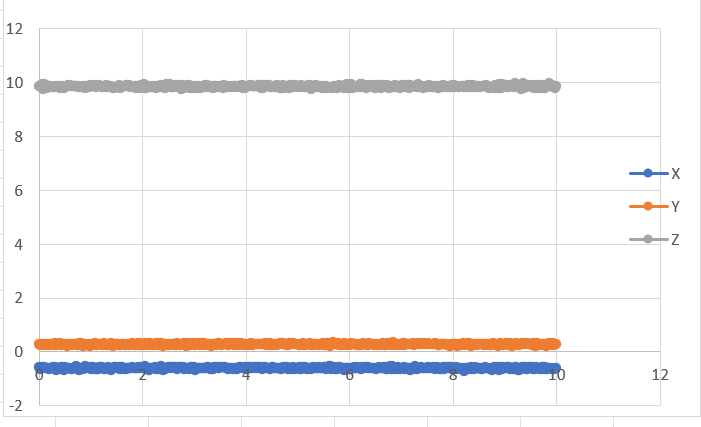
\includegraphics[width=6.5cm]{figures/accelero-afb/waardenSchermBoven.png}
\end{SCfigure}
Wat meteen opvalt bij het kijken naar deze output is de ruis; er is duidelijk een niet verwaarloosbare hoeveelheid ruis aanwezig. Dit is een logisch fenomeen; elk object op aarde trilt continu.
Op ruwe data zal bijgevolg steeds een bepaalde hoeveelheid ruis zitten.

\section{Oriëntatie van de assen}
%
%\begin{wrapfigure}{l}{5.0cm}
%\begin{center}
    %\label{wrap-fig:2}
    %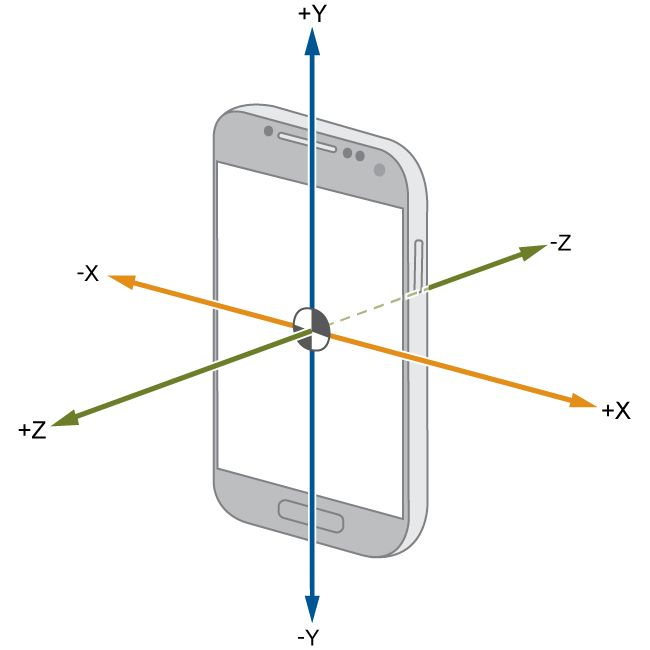
\includegraphics[width=4.0cm]{figures/accelero-afb/assenstelsel.JPG}
    %\caption{Oriëntataie van de assen}
%\end{center}
%\end{wrapfigure}
Wanneer het toestel in andere posities wordt geplaatst, zal de uitvoerwaarde verschillen, en zal aan de hand van de nieuwe output de oriëntatie van de assen kunnen worden bepaald.
Figuur 1.2 geeft de bevindingen weer.

\begin{SCfigure}[0.5][h]
\caption{Oriëntataie van de assen}
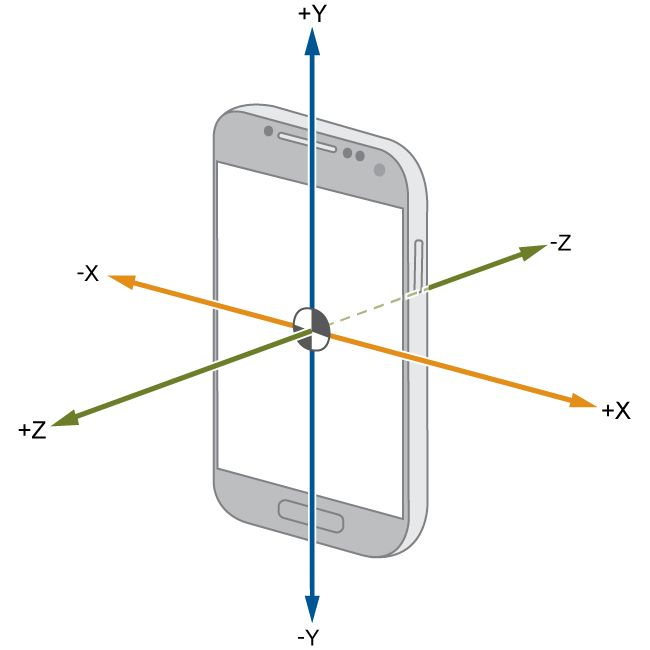
\includegraphics[width=4.5cm]{figures/accelero-afb/assenstelsel.JPG} 
\end{SCfigure}

\section{Output onder invloed van een hoek}
De outputwaarden voor de verschillende assen zijn zeer afhankelijk van de hoek waarin het toestel zich bevindt. Met \ref{eq:1} en \ref{eq:2} wordt de versnelling langs de assen (in $\frac{m}{s^2}$) gevonden.

\begin{equation}\label{eq:1}
	s_{z} &= s_{tot } \cdot \cos{(\alpha)} 
\end{equation}
\begin{equation}\label{eq:2}
	s_{y} &= s_{tot} \cdot \sin{(\alpha)} 
\end{equation}
\begin{SCfigure}[0.4][h]

\caption{Verduidelijking vergelijkingen }
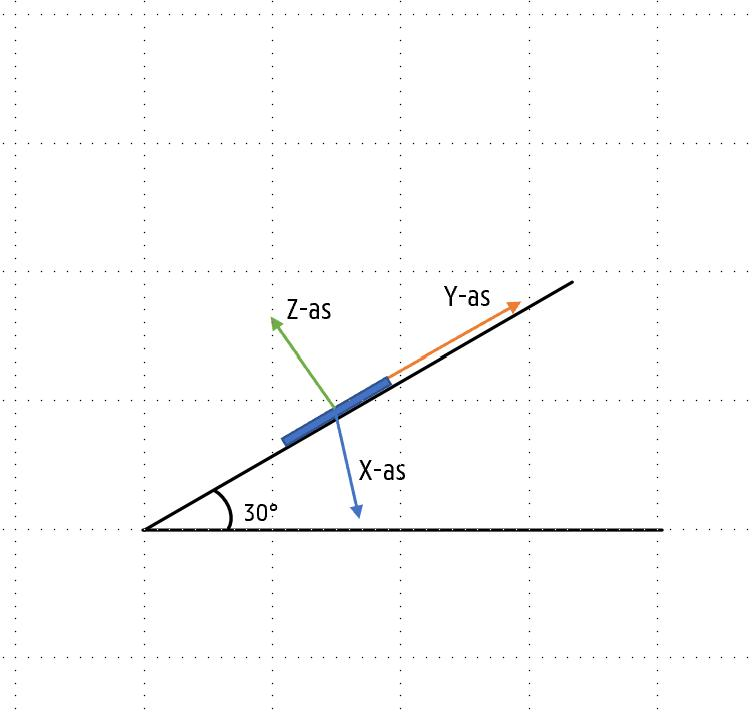
\includegraphics[width=.6\linewidth]{figures/accelero-afb/tafb.JPG}
\end{SCfigure}

Met $\alpha$ als de hoek tussen het toestel en het aardoppervlak. $s$ is de gebruikte variabele omdat over versnelling wordt gesproken. Er staan nu formules voor $z$ en $y$, maar het toestel kan gedraait worden om de $x$-waarden te vinden. In Figuur 1.3 worden de vergelijkingen visueel ondersteund. Hoe $s_{tot} $ berekend wordt, is verduidelijkt in \ref{eq:3}.

\section{Van 3D naar 1D}
Met al deze gegevens werken is mogelijks lastig en onduidelijk. De drie versnellingen moeten tot één enkele versnelling worden omgevormd, door gebruik te maken van de afstandsformule zoals weergegeven in 1.3.
\begin{equation}\label{eq:3}
	s_{tot} &= \sqrt{s_{x} ^2+s_{y} ^2+s_{z} ^2}  
\end{equation}

Hierbij moeten geen zorgen gebaard worden wat betreft dataverlies; het enige relevante om stappen te bepalen is de totale versnelling $s_{tot} $.
Figuur 1.4 toont een output na het zetten van 10 stappen omgezet naar totale versnelling.

\begin{SCfigure}[0.5][h]
\label{fig:4}
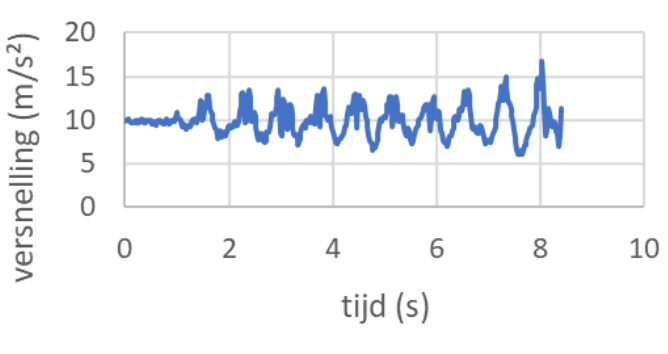
\includegraphics[width=6.5cm]{figures/gemiddelden/ruweData.png} 
\caption{Onbewerkte output totale versnelling}
\end{SCfigure}

Merk op dat er ongewenst veel ruis, kleine pieken, in deze grafiek zitten. Dit zou problemen kunnen veroorzaken, aangezien stappen tellen eigenlijk neerkomt op het tellen van deze pieken.
\section{Ruis aanpakken}
Om de ruis kwestie zo goed mogelijk aan te pakken, wordt gebruik gemaakt van bepaalde technieken om gegevens te verwerken.
Twee technieken werden bekeken; lopend gemiddelde en gewogen gemiddelde.
\subsection{Lopend gemiddelde}
Voor een lopend gemiddelde worden minstens twee opeenvolgende elementen genomen en wordt daar het gemiddelde van genomen tot vorming van een nieuw element. Dat nieuw element komt op de grafiek van het lopend gemiddelde. 
Hierbij kunnen deze opeenvolgende termen waarden voor of na het huidige element zijn. 
Het kan ook dat enkele elementen ervoor en enkele elementen na het huidige element liggen. 
Het lopend gemiddelde berekend voor twee elementen wordt beschreven door 1.4.
\begin{equation}\label{eq:4}
s_{i, lg} &= \frac{s_{i+j}+s_{i+j+1}  }{2 } 	
\end{equation}
Daarbij is $s_{i,lg} $ het nieuwe lopend gemiddelde element met index i. $s_{i+j} \text{ en } s_{i+j+1}  $ zijn datapunten uit de grafiek van de totale versnelling.
De index wordt op die manier geschreven, om erop te wijzen dat de elementen gekozen worden afhankelijk van i. Kies $j<0$ om elementen voor i te gebruiken. Kies $j&= 0  $ om gebruik te maken van datapunt i en de opeenvolgende. 

\\ Dit moet niet perse met twee elementen gebeuren, er blijft zo namelijk nog te veel ruis over.
Algemeen wordt het lopend gemiddelde als bij \ref{eq:5} neergeschreven. 
\begin{equation}\label{eq:5}
	s_{i,lg} &= \frac{s_{i+j} + s_{i+j+1} + \ldots+s_{i+j+n} }{N} \\
\end{equation}
Waarbij $N$ naar het aantal elementen verwijst. Hier zou dit $n+1$ zijn.
Dit kan meer compact geschreven worden.
\begin{equation}\label{eq:6}
	\equiv s_{i,lg} &= \frac{1}{N}\sum_{x=0}^{N-1} s_{i+j+x}  
\end{equation}
Waarbij de keuze van j dus te bepalen valt. 

\subsection{Gewogen gemiddelde}
Bij een gewogen gemiddelde gebeurt exact hetzelfde als bij het lopend gemiddelde, maar een factor $q$ wordt met ieder element vermenigvuldigd. De som van alle factoren $q$ is gelijkk aan één. Op deze manier worden bepaalde waarden zwaarder doorgewogen dan anderen, vandaar de naam "gewogen gemiddelde".
\begin{equation}\label{eq:7}
	s_{i,gg} &= \frac{1}{N} \sum_{j=0}^{N-1} q_{j} \cdot s_{i+j+x} \,\,\,\,\,\, |\,\,\, \sum_{j=0}^{N-1} q_{j} &= 1   
\end{equation}

\subsection{Uiteindelijke keuze voor gegevensverwerking}
Naarmate een hoger aantal elementen gekozen wordt om mee te werken, kost dit het toestel een stuk meer energie. Er moet een evenwicht gevonden worden. Er is nood aan duidelijke data zonder ruis, maar de app moet efficiënt blijven.
Het viel op dat de verkregen grafiek bij een gecentreerd lopend gemiddelde met elf elementen goed werkt. Dit zorgt niet voor een te grote hoeveelheid calculaties die moeten worden verricht. Desondanks levert het een grafiek op met minder ruis. 
\begin{equation}\label{eq:8}
	s_{i,lg} &= \frac{1}{11} \sum_{j=0}^{10} s_{i+j-5}  
\end{equation}
Er werd dus gewerkt met \ref{eq:8}. 
Figuur 1.5 toont de nieuw verkregen output.

\begin{SCfigure}[0.5][h]
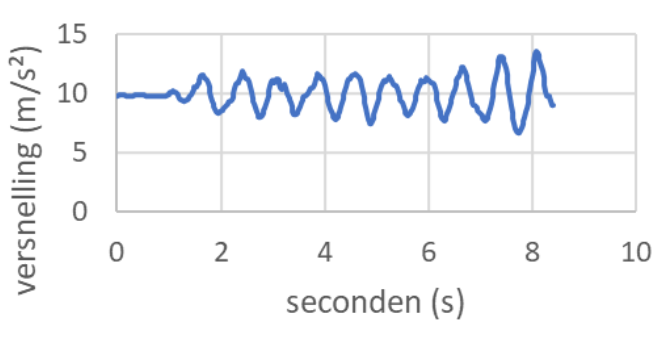
\includegraphics[width=6.5cm]{figures/gemiddelden/lopendGemiddelde.png} 
\caption{Gecentreerd lopend gemiddelde van 11 elementen}
\end{SCfigure}

Het gewogen gemiddelde had een zeer gelijkaardige output. Het lijkt eerder onnodig zaken extra moeilijk te maken door met een extra factor q te vermenigvuldigen. We maakten geen gebruik van deze techniek.

%%%%%%%%%%%%%%%%%%%%%%%%%%%%%%%%%%%%%%%%%%%%%
\chapter{\Large{Detectiemechanisme}}
Het doel van de stappenteller is uiteraard om het correct aantal stappen weer te geven. Dit is het kerndoel van de app. 
Om hierin te slagen zijn er meerdere detectoren gemaakt en getest door legio metingen. 
Zo is de beste detector voor de diverse bekeken bewegingen - contexten - gevonden.
De bekeken contexten zijn: toestel in de hand, broekzak, jaszak, achterzak.

\section{Implementatie lopend gemiddelde}

Er wordt natuurlijk begonnen met een lege lijst totale versnelling waarden. De eerste zes datapunten die gemeten worden, worden omgerekend naar hun totale versnelling en in een lijst gezet. 
Pas na deze zes waarden er zijn zal er dus een lopend gemiddelde kunnen berekend worden - de eerste waarden van de grafiek zijn dus een gemiddelde van zes, niet van elf waarden, aangezien de vijf eerdere waarden nog niet bestaan.
Zoals besproken in 1.1 wordt de UI sample rate gebruikt met een output van duizend waarden per minuut. 
Het duurt dus slechts iets meer dan een derde van een seconde om deze zes waarden te verkrijgen, verwaarloosbaar weinig. 
Praktisch onmiddellijk kunnen er stappen geteld worden door op die manier te werken, zorgen over een trage respons zouden overbodig zijn.
Vanaf elf waarden verkregen zijn, wordt er telkens een element verwijderd in het begin, en toegevoegd aan het einde.\\
Visueel wordt na zes datapunten een lijst zoals hieronder verkregen.
\[
s_{1} \,\,\,\,\,\, |\,\,\, s_{\ldots} \,\,\,\,\,\, |\,\,\, s_{6} 
.\] 
Hiermee wordt de output voor $s_{1,lg} $ berekend, waarbij met de $s_{i} $ datapunten van totale versnelling bedoeld worden. Na elf datapunten wordt dan de onderstaande lijst verkregen.
\[
s_{1} \,\,\,\,\,\, |\,\,\, s_{\ldots} \,\,\,\,\,\, |\,\,\, s_{11} 
.\] 
Daarmee wordt het gemiddelde voor $s_{6,lg} $ genomen.
Vanaf datapunt $s_{12} $ er is, wordt een lijst als hieronder verkregen.
\[
s_{2} \,\,\,\,\,\, |\,\,\, s_{\ldots} \,\,\,\,\,\, |\,\,\, s_{12} 
.\] 
Dit voor het element $s_{7,lg} $.
Dit proces blijft zich herhalen terwijl stappen geteld worden door te kijken naar de nieuwe output.

\section{Dit algoritme in pseudocode}
\begin{algorithm}[H]
\KwIn{Output van de accelerometer}
\KwOut{Lijst om het lopend gemiddelde mee te maken}

\SetAlgoLined
\SetNoFillComment
\vspace{3mm}

$s_{tot} $ = list(totale versnelling 1, totale versnelling 2, ...)

elementsInList = len($s_{tot} $)

listForMeanAverage = list()

\uIf{ $\text{elementsInList} < 11$ } {
	listForMeanAverage.append(nieuwste element in $s_{tot} $)
}
\Else {
	listForMeanAverage.remove(oudste element in de lijst)
	listForMeanAverage.append(nieuwste element in $s_{tot} $)
}

\Return listForMeanAverage\
\caption{ Hoe de lijst voor lopend gemiddelde wordt gemaakt in pseudocode}
\end{algorithm}

De elementen die $s_{tot} $ opmaken worden berekend als in \ref{eq:3}; het eerste datapunt - een x, y en z versnelling - wordt hiermee omgezet en is het eerste element in die lijst.


\section{Dummydetector}

Dit was onze eerste, eerder primitieve, stappendetector.
Het controleerde of het lopend gemiddelde boven een bepaalde grenswaarde kwam en indien dit het geval was werd er een stap geteld. 
Vervolgens wacht de detector tot het lopend gemiddelde er opnieuw onder zakt, vanaf dan herhaalt het proces zich en kan het een nieuwe stap tellen indien de grenswaarde wordt bereikt. Op die manier worden in essentie de pieken van de grafiek geteld. Het tellen van die pieken is eigenlijk het overkoepelende idee van een stappendetector.
Om dit te doen wordt onze grenswaarde op $5 $ - proefondervindelijk bepaald - gelegd.
In algoritme 2 wordt deze waarde CF genoemd, voor "constant function".

\begin{algorithm}[H]
\KwIn{Lopend gemiddelde}
\KwOut{Aantal stappen}

\SetAlgoLined
\SetNoFillComment
\vspace{3mm}

lg = (een gemiddelde van totale versnellingen)\\
Control = 0 \\
Steps = 0 \\
CF = 5 \\ 
\tcc{Onderstaande code wordt herhaald telkens er een nieuw element lg is.}
\uIf{ $lg > CF$ and $\text{Controle} = 0$ } {
Control = 1\\
Steps $++$\\
}
\uIf{ $i < CF$ } {
	Control = 0
}
\Return Aantal stappen;
\caption{ Dummydetector algoritme}
\end{algorithm} 
Dit principe is heel simplistisch, en gaf desondanks voor de meeste bewegingen al een relatief goed resultaat. Echter gaf het voor bepaalde bewegingen een totaal verkeerd beeld. 
Dit wordt later met diepgang besproken (Hoofdstuk 4).
 

\section{Complexe detector}

Uit de eerste labsessies bleek dat het verschil in versnelling tussen stappen met het toestel in de hand tegenover 
lopend met het toestel in de broekzak zeer groot is. Te groot om met een gemiddelde grenswaarde voor beide een goed resultaat te 
krijgen. 
De stappenteller moest dus op een of andere manier weten welke beweging de gebruiker aan het maken is. 
Dit probleem wordt aangepakt door de maximumwaarde variabel te maken. We schrijven een dynamische detector die de maximumwaarde opnieuw zal berekenen voor elke 400 waarden. Met deze nieuwe methode zou de grens zeer snel correct aangepast worden.
Dit is het hoofdprincipe dat de nieuwe dynamische detector onderscheidt van de dummydetector, maar daarnaast is er nog één extra verandering tegenover de dummydetector. 
Stel het toestel wordt op tafel geplaatst voor een minuut en vervolgens opgepakt voor een wandeling; de drempelwaarde is nu zeer laag. 
Er zullen meerdere ongezette stappen geteld worden tot de grens opnieuw is veranerd. Om dit tegen te gaan moet de waarde gebruikt om de drempelwaarde te berekenen groter zijn dan twee plus de versnelling in rust.
Er werd eerst drie in plaats van twee gekozen, maar dan ondstonden moeilijkheden bij testen met het toestel vlak in de hand.
%%%%%%%%%%%%%%%%%%%%%%%%%%%%%%%%%%%%%%%%%%%%%%%
\chapter{\Large{Mobiele applicatie}}
	
Voor het schrijven van de Android app werd een applicatie van de begeleiders waarin een eerste basis reeds geschreven stond, ter beschikking gesteld. Deze is voorzien van twee tabbladen; een tabblad waar de stappen moesten worden weergegeven en een tabblad waar de accelerometer output opgeslagen wordt. Vervolgens werd de app uitgebreid met het eerder besproken algoritme, het aantal stappen, het aantal calorieën, afgelegde afstand en een progressiecirkel.$^{[1]} $
Oorspronkelijk was er ook de ambitie om meer toepassingen te implementeren, maar omwille van de beperkte tijd is niet alles verwezelijkt. 

\begin{SCfigure}[0.5][!h]
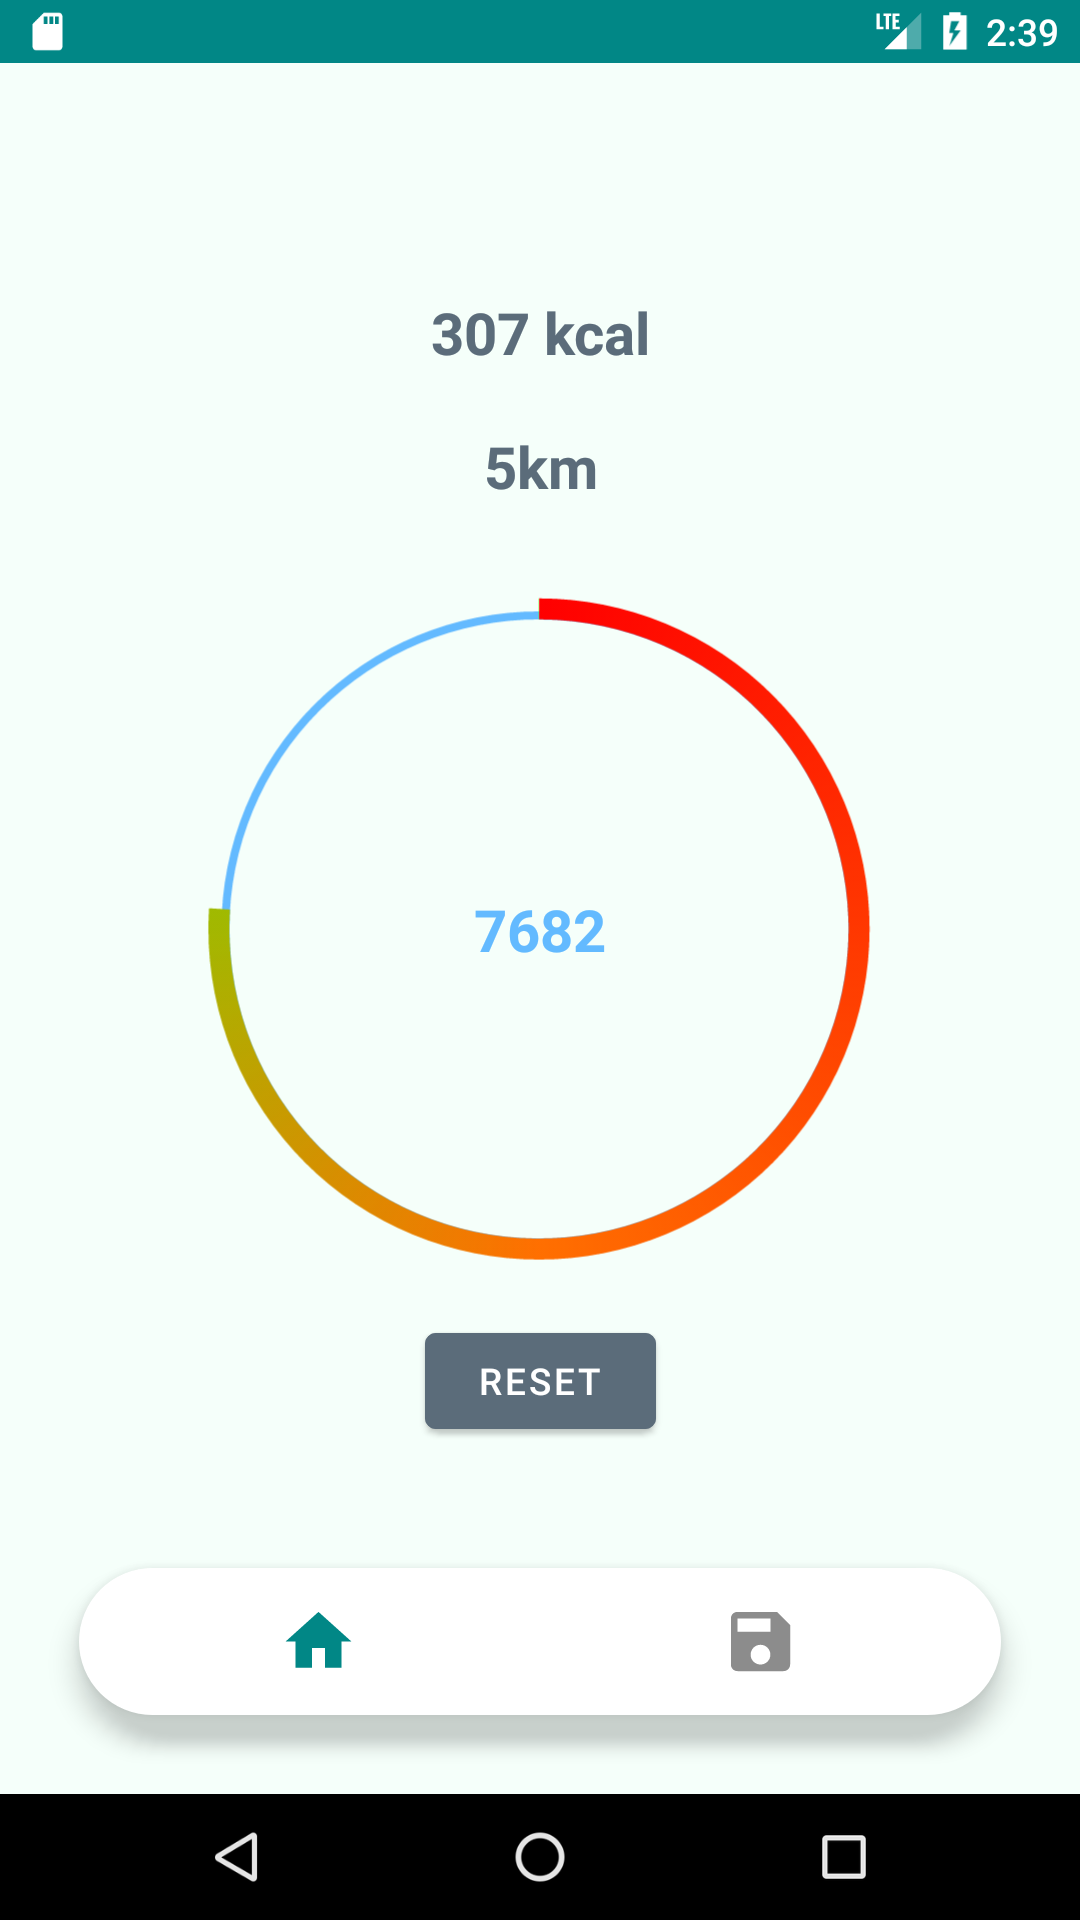
\includegraphics[width=3.5cm]{figures/progressiecirkel.png} 
\caption{Screenshot van de applicatie}
\end{SCfigure}

\section{Android Studio}
Voor het schrijven van de applicatie werd de programmeeromgeving Android Studio gebruikt. Android Studio is de officiële omgeving voor het ontwikkelen van Android-applicaties. Deze programmeeromgeving simuleert Android-apparaten op een computer, zodat toepassing op verschillende apparaten en Android API-niveaus kunnen getest worden zonder dat een fysiek apparaat nodig is. De code wordt geschreven in Java. 
 
\section{Aantal stappen weergeven}
Het aantal stappen is een object dat zichtbaar is op de UI. Dit houdt in dat het aantal stappen wordt weergegeven als een “TextView”.$^{[2]} $ Een TextView is een Android gebonden object dat bedoeld is voor het weergeven van tekst en optioneel het bewerken van tekst door de gebruiker. Een TextView wordt aangemaakt in de grafische editor van Android Studio. Vervolgens is deze gelinkt met de code, zodanig dat bij iedere stap die geregistreerd wordt dit aantal met één verhoogd wordt.  
\section{Aantal calorieën weergeven}
Het aantal calorieën wordt op analoge manier weergegeven in de UI. Dit aantal wordt berekend afhankelijk van het aantal stappen, dit via het lineair verband dat stelt dat iedere stap 0.04 calorieën is.$^{[3]} $  
\section{Afgelegde afstand weergeven}
Net zoals het aantal calorieën werd de afgelegde afstand op analoge wijze geïmplementeerd. De afgelegde afstand is ook een lineair verband, waarbij 1333 stappen het equivalent zou zijn van één kilometer.$^{[4]} $
\section{Progressiecirkel weergeven}
Android Studio beschikt zelf over een ingebouwde progressiecirkel. Standaard is deze progressiecirkel ingesteld als een cirkelvormige laadbalk die blijft ronddraaien zolang er een bewerking bezig is, net zoals vaak op populaire apps wordt gedaan. Na het programmeren van de progressiecirkel en de functionaliteit te veranderen naar het weergeven van progressie, bleek de progressiecirkel niet langer cirkelvormig te zijn, maar balk vormig. De cirkelvorm moeten worden gecreëerd via een XML-bestand als drawable bron. Een drawable bron is een algemeen concept voor een afbeelding of object die op het scherm kan worden weergegeven. Zo'n bron kan op verschillende objecten worden toegepast, zodanig dat deze slechts eenmalig dient gedefiniëerd te worden. Voor het creëren van de progressiecirkel werden twee van zulke bronnen gedefinieerd, voor de cirkelvorm en voor de kleuren. De progressiecirkel verkleurt ook naarmate er meer stappen worden gezet, beginnend bij donkerrood waarna hij telkens groener kleurt. 
Dit natuurlijk omdat mensen de kleur rood associëren met "slecht, het doel is niet voltooid", en groen daaraantegen met "goed, het doel is voltooid".
\section{Bespreking van de code}
De volledige app bestaat uit verschillende classes. Er zijn drie classes gelinkt aan het hoofdscherm. Zo is er bijvoorbeeld “HomeFragment” dit is waar de calorieën, de totale afstand en progressiecirkel worden weergegeven. Er is ook een class genaamd “BetereDetector” en “DummyDetector”, BetereDetector is de class waar het algoritme is geschreven dat stappen telt. DummyDetector was één van onze eerste algoritmes voor het tellen van stappen, deze is minder nauwkeurig en wordt dan ook niet meer gebruikt in de app, zoals eerder al besproken. Deze class staat nog in de code omdat voor het testen de beide detectoren moesten worden vergeleken. Op die manier kan snel gewisseld worden tussen detectoren.
\section{Reset knop weergegeven}
De reset knop is een object genaamd “Button”. Dit is een object waarop gedrukt kan worden die in respons een voorop geprogrammeerde functie uitvoert. In ons programma zet deze knop het aantal stappen terug op nul, net zoals de afstand, aantal calorieën en de progressiecirkel. Het idee is dat gebruikers dan bij het aanvangen van een nieuwe dag, of eender welk moment naar keuze de teller opnieuw kunnen laten beginnen. 
%%%%%%%%%%%%%%%%%%%%%%%%%%%%%%%%%%%%%%%%%%%%%%%
\chapter{\Large{Resultaten}}
Na afloop van de labsessies is er nu een UI met functionerende stappenteller. De grootst gemeten foutmarge is 6 procent. 
\section{Resultaten van de detectoren}
Hoe accuraat de detector is, hangt af van de manier waarop het toestel wordt vastgehouden. De onderstaande tabellen tonen de exacte bevindingen met onze twee detectoren voor verschillende manieren waarop het toestel kan worden vastgehouden.

Dit deel is beperkt tot het toestel in de broekzak en jaszak, aangezien hiermee interessante gegevens werden verkregen om te vergelijken.

\subsection{Toestel in broekzak}

\begin{tabular}{ |p{2.5cm}||p{4cm}|p{3cm}|p{3cm}|  }
 \hline
 \multicolumn{2}{|c|}{Tabel 4.1: Toestel in broekzak} \\
 \hline
 Dynamische detector& Statische detector \\
 \hline
 52   & 46   \\
 51&   48  \\
 49 &45 \\
 48&45 \\
 \hline
\end{tabular}
\\ 
\\Het rekenkundig gemiddelde wordt gegeven door 4.1.
\begin{equation}\label{eq:9}
AM &= \frac{1}{N} \sum_{i=1}^{N} a_{i} &= \frac{a_{1} +a_{2} +\ldots+a_{N} }{N}     	
\end{equation}
De $AM$ komt van de Engelse term; arithmetic mean.
Dit wordt toegepast op de bevindingen.
\begin{itemize}
	\item Toegepast op de dynamische detector: $AM_{dy} &= 50 $
	\item Toegepast op de statische detector: $AM_{st} &= 46 $
\end{itemize}

De root mean squared error wordt gegeven door 4.2.
\begin{equation}\label{eq:10}
	RMSE &=  \sqrt{\frac{1}{N}\sum_{i=1}^{N} (\hat{\theta}_{i} - \theta _{i}   )^2} 
\end{equation}
Hierbij is $\hat{\theta}$ het aantal gemeten stappen en $\theta $ het aantal gezette stappen.
\begin{itemize}
	\item Toegepast op de dynamische detector: $RMSE_{dy} &= \sqrt{2,5}  $
	\item Toegepast op de statische detector: $RMSE_{st} &= \sqrt{17,5}  $
\end{itemize}
Deze formules - 4.1 en 4.2 - toepassen op data is interessant om resultaten beter te kunnen interpreteren.

\subsection{Toestel in de jaszak}

\begin{tabular}{ |p{2.5cm}||p{4cm}|p{3cm}|p{3cm}|  }
\hline
\multicolumn{2}{|c|}{Tabel 4.2: Toestel in jaszak} \\ \hline
Dybamische detector& Statische detector\\
\hline
52   & 26   \\
50&   25  \\
49 &23 \\
48    & 27\\
\hline
\end{tabular}
\\ \\ 
Hier worden eveneens de bewerkingen van 4.1 en 4.2 toegepast. 
\begin{itemize}
	\item Toegepast op de dynamische detector:  $AM_{dy} &= 49,75 $ en $RMSE_{dy} &= \sqrt{2,25}  $
	\item Toegepast op de statische detector: $AM_{st} &= 45,25 $ en $RMSE_{st} &= \sqrt{614,75}  $
\end{itemize}

\section{Bespreken van deze bevindingen}
Zoals te zien in tabel 1.1 is de statische detector - dummydetector - nog behoorlijk correct met het toestel in de broekzak, met een rekenkundig gemiddelde van 46. Dit omdat elke stap zeer duidelijke pieken oplevert. Toen de detector voor het eerst gestest werd - met het toestel in de achterzak - werden altijd bijna perfecte resultaten met een zeer laag foutmarge gevonden. De resultaten wanneer het toestel in de hand gehouden wordt of in de jaszak gestopt wordt daaraantegen, zijn een stuk minder accuraat. De dynamische detector zorgt voor lagere foutmarges in elke context.

\section{Vergelijking met een andere applicatie}

De stappenteller applicatie zoals hier geschreven, is vergeleken met een betalende uit de Play Store; StepsApp.$^{[5]} $
 De keuze van deze specifieke applicatie om tegen te testen is gemaakt aangezien StepsApp bovenaan stond in de app store, en meer dan 20 miljoen downloads heeft. De app is in principe betalend, dus moest een free trial gestart worden.
 Deze werd vergeleken met onze dynamische detector, dit is namelijk de detector gebruikt in onze applicatie. 
 Het toestel wordt in de hand gehouden, aangezien dat de moeilijkste test is met de meeste fouten.
 Het rekenkundig gemiddelde en de root mean squared error worden op de data toegepast om goed te kunnen vergelijken.

 \begin{tabular}{ |p{2,5cm}||p{4cm}|p{3cm}|p{3cm}|  }
 \hline
 \multicolumn{2}{|c|}{Tabel 4.3: Toestel in hand.} \\
 \hline
 StepsApp resultaten& Onze dynamische detector resultaten.\\
 \hline
57    &   47 \\
50 &  50   \\
 48 & 51\\
  54   & 49\\
 \hline
 \end{tabular}
 \[
 AM_{StepsApp} &= 53 \text{ en } RMSE_{StepsApp} &= \sqrt{69}  
 .\] 
 \[
 AM_{dy} &= 49,25 \text{ en } RMSE_{dy} &= \sqrt{2,75}   
 .\] 


 Natuurlijk had de StepsApp wel een meer uitgebreide interface en allerlei andere opties, maar na vijf testen lijkt het hier ontwikkelde dynamische algoritme voor superieure resultaten te zorgen. Het is niet uitgesloten dat met meer uitgebreide testen andere resultaten hadden bekomen.
%%%%%%%%%%%%%%%%%%%%%%%%%%%%%%%%%%%%%%%%%%%%%%

\onecolumn
\begin{thebibliography}{99}

\bibitem{1} 
“Material Design for Android,” Android Developers.\\ 
\url{ https://developer.android.com/develop/ui/views/theming/look-and-feel}\\  (Geraadpleegd 12 Dec. 2022).​

\bibitem{2} 
\textit{"Styles and Themes,"}
Android Developers\\ 
\url{https://developer.android.com/develop/ui/views/theming/themes}\\  (Geraadpleegd 12, Dec. 2022).​

\bibitem{3}
"Stappenchallnge of geen stappenchallenge, that's the question"
foodlive.nl \\
\url{https://www.foodilove.nl/10-000-stappen/#:~:text=Afhankelijk%20van%20je%20gewicht%20verbrand,calorie%C3%ABn%20per%20dag%20door%20beweging.}
(Geraadpleegd 20, Dec. 2022)

\bibitem{4}
“Aantal stappen omzetten naar kilometers - Hardlopen,” Wim Groenendijk.\\ 
\url{https://www.groenendijkwim.nl/hardlopen/stappen-naar-kilometers/#:~:text=Hoeveel%20stappen%20is%20een%20kilometer} \\ (Geraadpleegd 12, Dec. 2022).​

\bibitem{5} 
“StepsApp,” steps.app, 2015.\\ 
\url{https://steps.app/nl} \\ (Geraadpleegd 06, Dec. 2022).​


\end{thebibliography}

\thispagestyle{empty}
\end{document}
Footer

